\iffalse
\documentclass[journal,10pt,twocolumn]{article}
\usepackage{graphicx}
\usepackage[margin=0.5in]{geometry}
\usepackage[cmex10]{amsmath}
\usepackage{array}
\usepackage{booktabs}
\usepackage{mathtools}
\usepackage{multicol}
\usepackage[utf8]{inputenc}
\title{\textbf{Conic section Assignment}}
\author{T.Varsha Reddy}
\date{September 2022}


\providecommand{\norm}[1]{\left\lVert#1\right\rVert}
\providecommand{\abs}[1]{\left\vert#1\right\vert}
\let\vec\mathbf
\newcommand{\myvec}[1]{\ensuremath{\begin{pmatrix}#1\end{pmatrix}}}
\newcommand{\mydet}[1]{\ensuremath{\begin{vmatrix}#1\end{vmatrix}}}
\providecommand{\brak}[1]{\ensuremath{\left(#1\right)}}
\providecommand{\lbrak}[1]{\ensuremath{\left(#1\right.}}
\providecommand{\rbrak}[1]{\ensuremath{\left.#1\right)}}
\providecommand{\sbrak}[1]{\ensuremath{{}\left[#1\right]}}

\begin{document}

\maketitle
\section{Problem Statement}
\fi
Find the equation of the tangent to the curve 
\begin{align}
	y = \sqrt{3x-2}
\end{align}
which is parallel to the line
\begin{align}
	4x-2y+5 = 0
\end{align}
\solution 
\iffalse
\section{Solution}
The given equation of parabola $y^2 = 3x-2$ can be written in the general quadratic form as
\begin{align}
    \label{12/6/3/25eq:conic_quad_form}
    \vec{x}^{\top}\vec{V}\vec{x}+2\vec{u}^{\top}\vec{x}+f=0
    \end{align}
where
\fi
The parameters for the given conic are
\begin{align}
	\label{12/6/3/25eq:V_matrix}
	\vec{V} &= \myvec{0 & 0\\0 & 1},
	\\
	\label{12/6/3/25eq:u_vector}
	\vec{u} &= \myvec{-3/2\\0},
	\\
	\label{12/6/3/25eq:f_value}
	f &= 2
	%\\
\end{align}
which represent a parabola. 
Following the approach in problem 
\ref{chapters/12/6/3/15},
\iffalse
Thus can be expressed as by choosing
\begin{align}
%\label{12/6/3/25eq:eta}
Ki = \frac{\vec{Pi}^T\vec{u}}{\vec{Pi}^T\vec{n}}
\end{align}
%\begin{center}
   where
   \fi
   \begin{align}
     \vec{p_1} &= \myvec{1\\0},
     \\
     \vec{n} &= \myvec{-2\\1},
    \end{align}
    \iffalse
   
%\end{center}
If V is non invertible,given the normal vector $\eta$,the point of contact is given by the matrix equation. 

\begin{align}
    \myvec{( \vec{u}+\vec{ki}\vec{n})^T\\ \vec{V}}\vec{q} &= \myvec{-f \\ (\vec{Ki}\vec{n}-\vec{u})}  &\abs{V} &= 0
    \label{12/6/3/25eq:conic_parab_c}
    \end{align}
Substituting appropriate values from \eqref{12/6/3/25eq:V_matrix}, \eqref{12/6/3/25eq:u_vector}, \eqref{12/6/3/25eq:f_value}, and into \eqref{12/6/3/25eq:conic_parab_c}, the below matrix equation is obtained
\fi
yielding the matrix equation
\begin{align}
	\label{12/6/3/25eq:vertex_system}
	\myvec{-3&0\\0& 0\\0& 1}\vec{q} = \myvec{-41/16\\0 \\3/4}\\
\end{align}
The augmented matrix for \eqref{12/6/3/25eq:vertex_system} can be expressed as
\begin{align}
	%\label{12/6/3/25eq:vertex_solv1}
	%\myvec{-3&0&\vrule&2\\0&0&\vrule&0\\0&1&\vrule&0}\\ 	
	%\label{12/6/3/25eq:vertex_solv2}
	\xleftrightarrow[]{R_2 \leftrightarrow R_3}\myvec{-3&0&\vrule&-41/16\\0&1&\vrule&0\\0&0&\vrule&3/4}\\
	\label{12/6/3/25eq:vertex_solv3}
	\xleftrightarrow[]{-\frac{R_1}{-3} \leftarrow R_2}\myvec{1&0&\vrule&41/48\\0&1&\vrule&0\\0&0&\vrule&3/4}\\
	\label{12/6/3/25eq:vertex_solv4}
	\implies\vec{q} = \myvec{\frac{41}{48}\\\frac{3}{4}}
\end{align}
The equation of tangent is then obtained as
\begin{align}
	\myvec{-2 & 1}\vec{x} +\frac{23}{24} = 0 
\end{align}
See Fig. 
		\ref{fig:12/6/3/25}.
	\begin{figure}[!h]
		\centering
 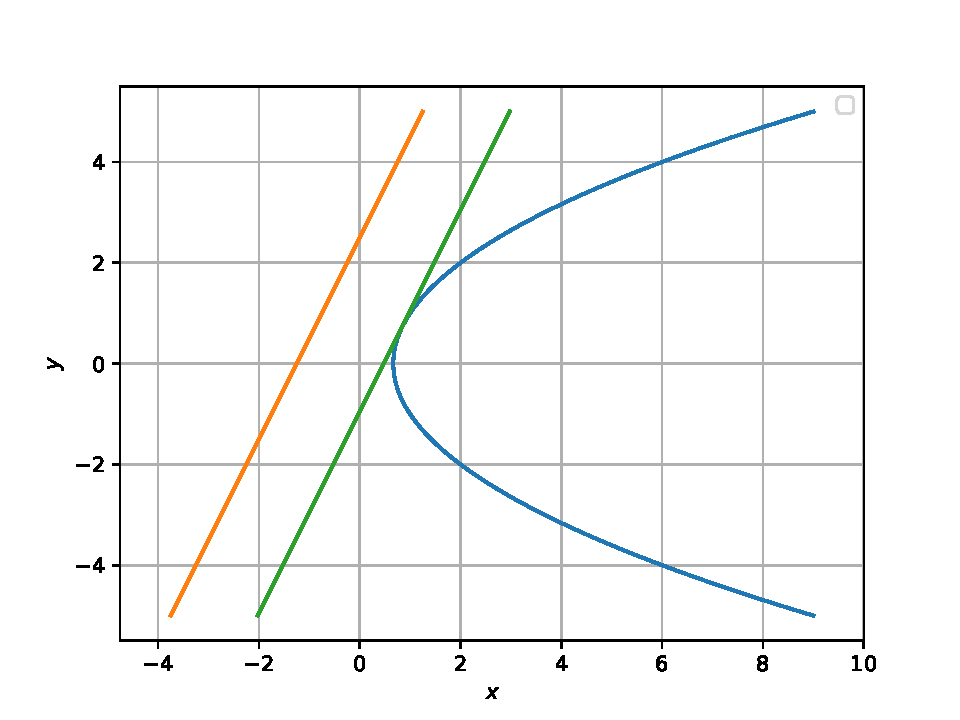
\includegraphics[width=\columnwidth]{chapters/12/6/3/25/figs/conic.pdf}
		\caption{}
		\label{fig:12/6/3/25}
  	\end{figure}
\iffalse
\begin{center}
\begin{align}
 \vec{(Vq+u)}^{\top}\vec{X}+\vec{u}^{\top}\vec{q}+\vec{f} =0 
\end{align}
\end{center}
\section{ Construction}
%\includegraphics[scale=0.5]{../Documents/co.pdf} 
%\includegraphics[scale=0.5]{co.pdf} 
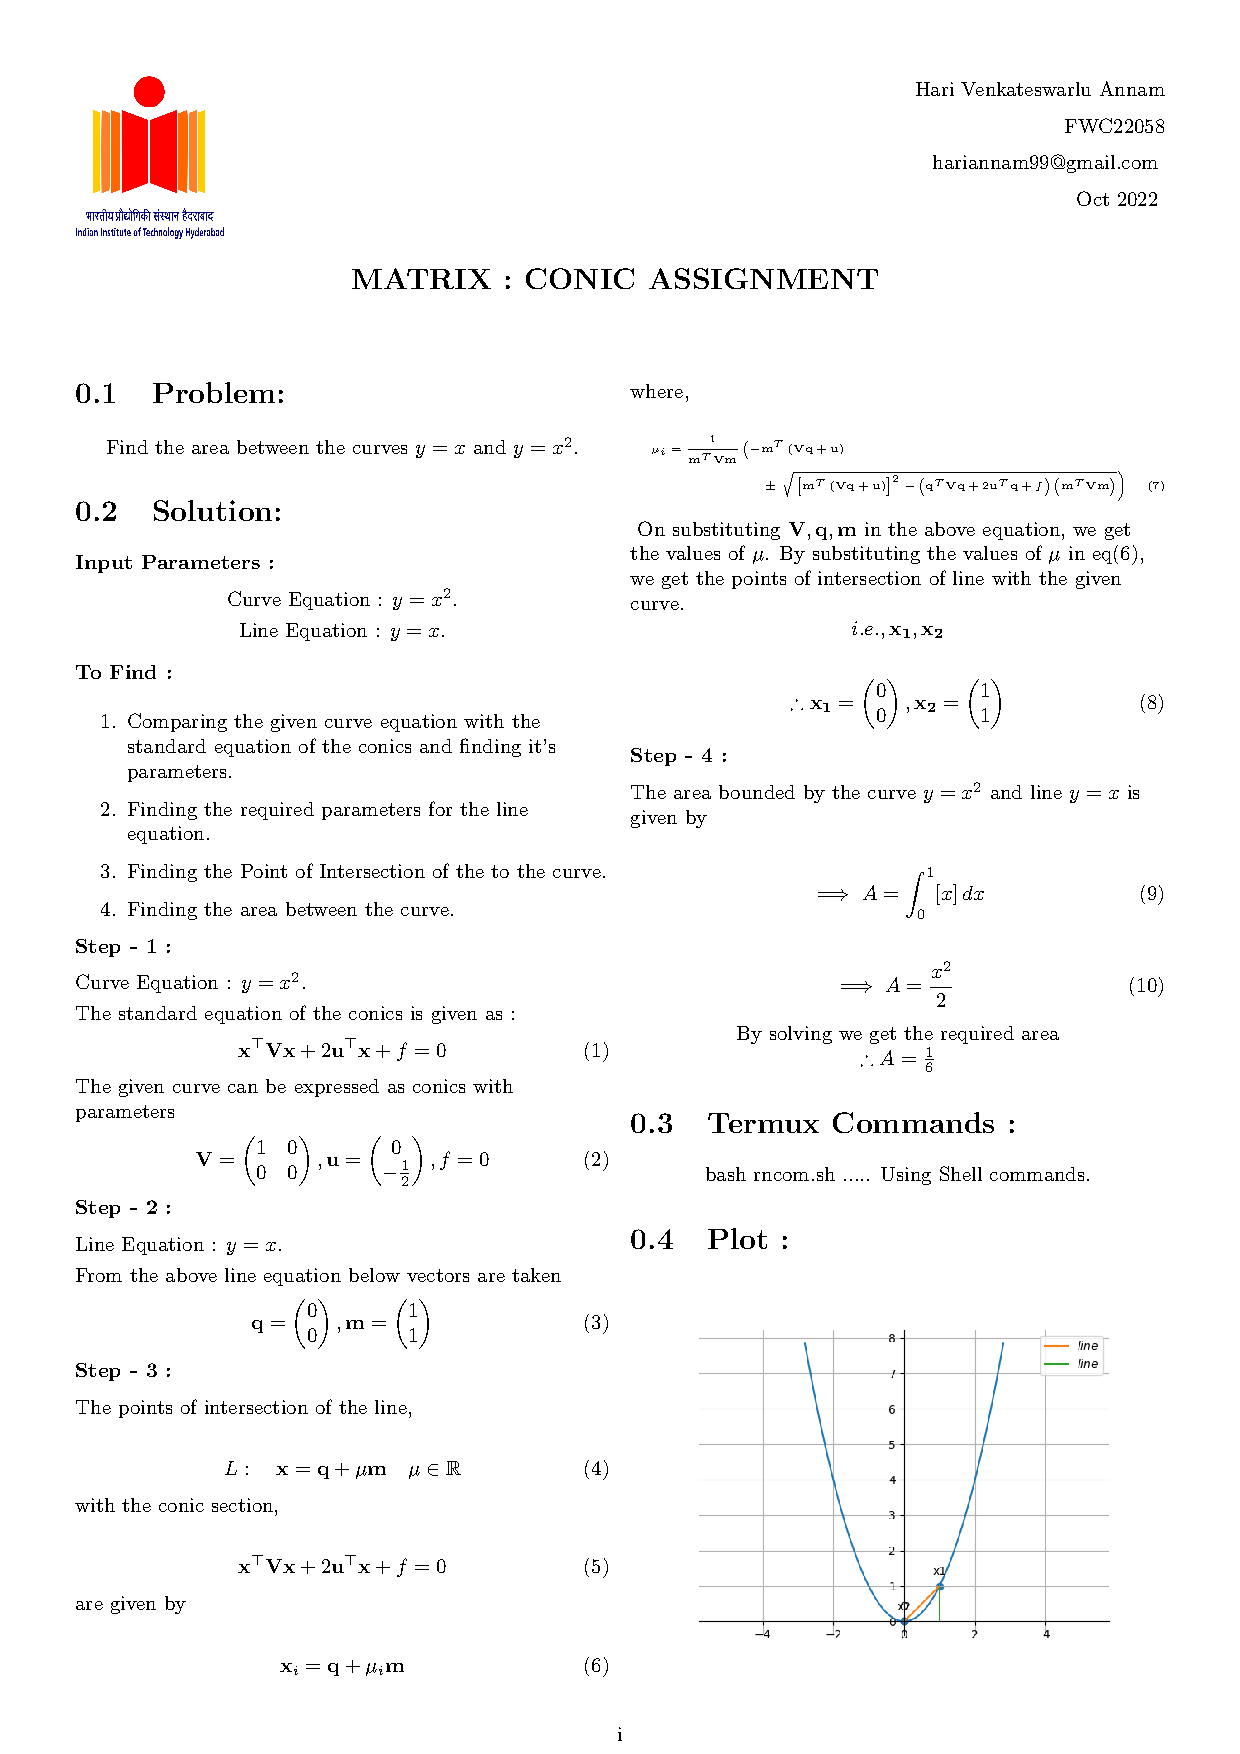
\includegraphics[scale=0.5]{conic.pdf} 
%\vspace{3mm}
%\url{https://github.com/9705701645/FWC/blob/main/co.py}
%\begin{multicols}
 %Download the code \\
%\href{https://github.com/9705701645/FWC/blob/main/co.py}{Assignment-5}.
%\end{multicols}
\end{document}


\fi
